\chapter{Generative Adversarial Networks (GANs)}

Before GANs, autoencoders and VAEs were major generative models. VAEs were a major breakthrough because they learned a continuous latent space, allowing them to generate new images by sampling latent vectors. However, they had a major drawback: the generated images were often blurry.

The main reason for this blur is the reconstruction loss, such as MSE or $L_1$ loss. During training, a VAE tries to reconstruct the original image pixel by pixel. When multiple outputs are possible, the safest way to minimize the reconstruction loss is to predict the average of all plausible images. Averaging pixels smooths edges and textures, producing blurry results.

Researchers realized that pixel similarity does not necessarily mean visual realism. Two real images of the same object can have very different pixel values because of lighting, pose, or background, yet both look perfectly realistic to humans.

This led to a new idea: instead of asking the model to reconstruct a specific image, ask it to generate an image that looks real. To achieve this, GANs introduced a second neural network called the discriminator, whose job is to distinguish real images from fake ones.

The generator learns to create fake images that fool the discriminator, while the discriminator learns to detect them. This competitive process is called adversarial learning.

The key innovation of GANs is that they optimize for realism rather than pixel accuracy, allowing them to generate much sharper and more realistic images than VAEs.

\begin{propertybox}[Summary: VAE vs. GAN]
\begin{itemize}
    \item \textbf{VAE}: Generates images using reconstruction loss $\rightarrow$ often blurry
    \item \textbf{Problem}: Pixel-wise losses encourage averaging, reducing image sharpness and blurring images
    \item \textbf{GAN Solution}: Replace reconstruction with adversarial learning
    \item \textbf{Generator}: Creates fake images
    \item \textbf{Discriminator}: Distinguishes real from fake images
    \item \textbf{Goal}: Generate images that look realistic enough to fool the discriminator
\end{itemize}
\end{propertybox}

\section{Vanilla GAN}

Unlike an autoencoder, a GAN does not have an encoder, a decoder, or a reconstruction loss. Instead, it has two completely different neural networks that compete against each other:
\begin{itemize}
    \item Generator ($G$)
    \item Discriminator ($D$)
\end{itemize}

This competition is what makes GANs unique.

\subsection*{I) The Generator}

The generator is responsible for creating images. Unlike an autoencoder, it does not receive an image; instead, it takes a random noise vector $z$ (usually sampled from a Gaussian distribution) and learns a mapping:

\[
z \longrightarrow \text{Generator} \longrightarrow \text{Fake Image}
\]

We start from random noise because we want the generator to create new images, not copy existing ones.

The input to the generator is usually written as $z \sim \mathcal{N}(0, 1)$, a random vector from a Gaussian distribution.
\[
z = [0.21, -1.34, 0.56, \dots]
\]
These numbers have no meaning. They are just random values. The generator's job is to transform meaningless noise into a realistic image.

\subsection*{II) The Discriminator}

The discriminator is a binary classifier. It receives either a real image from the dataset or a fake image generated by the generator and outputs the probability that the image is real.

\[
\text{Image} \longrightarrow \text{Discriminator} \longrightarrow \text{Probability} \longrightarrow \begin{cases} \text{Real} \\ \text{or} \\ \text{Fake} \end{cases}
\]

\begin{itemize}
    \item $0.98 \rightarrow 98\%$: This is likely a real image.
    \item $0.02 \rightarrow$: This image is almost certainly fake.
\end{itemize}

The discriminator receives two kinds of images:
\begin{itemize}
    \item \textbf{Real image}: These come directly from the training dataset.
    \item \textbf{Fake image}: These come from the generator.
\end{itemize}

The discriminator never knows which one it receives. Its only task is to answer: real or fake?

\subsection*{Architecture}

\begin{figure}[H]
\centering
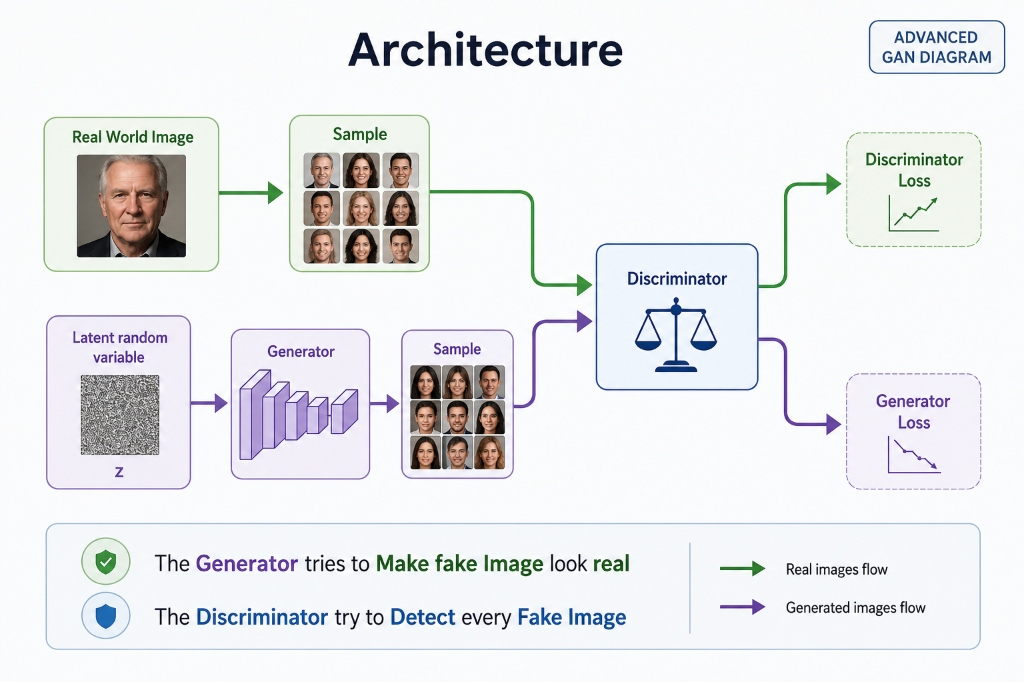
\includegraphics[width=0.88\textwidth]{figures/fig_9_1_advanced_gan_architecture.jpg}
\end{figure}

\begin{itemize}
    \item The \textbf{generator} tries to \textbf{make fake images look real}.
    \item The \textbf{discriminator} tries to \textbf{detect fake images}.
\end{itemize}

\section{The Training Process}

\begin{enumerate}
    \item Sample a batch of real images from the dataset.
    \item Sample a batch of random noise vectors $z$.
    \item Generate fake images using the generator:
    \[
    \text{Fake Images} = G(z)
    \]
    \item Train the Discriminator using:
    \begin{itemize}
        \item Fake images (from the generator) $\rightarrow$ target = fake ($0$)
        \item Real images $\rightarrow$ target = real ($1$)
        \item Update only the discriminator.
    \end{itemize}
    \item Sample another batch of random noise (or reuse the previous one).
    \item Generate fake images again $G(z)$
    \item Freeze the Discriminator's weights (so they are not updated)
    \item Pass the fake images through the discriminator.
    \item Update only the generator so that the discriminator classifies its fake images as real ($1$).
    \item Repeat.
\end{enumerate}

Generate fake images twice because the generator changes after every update:
\begin{itemize}
    \item The first fake batch is used to train the discriminator.
    \item The second fake batch is used to train the generator while the discriminator is frozen.
\end{itemize}

Some implementations reuse the same fake images, while others generate a new batch. Both approaches work; generating a new batch is common.

\subsubsection*{Training the Discriminator}

\begin{figure}[H]
\centering
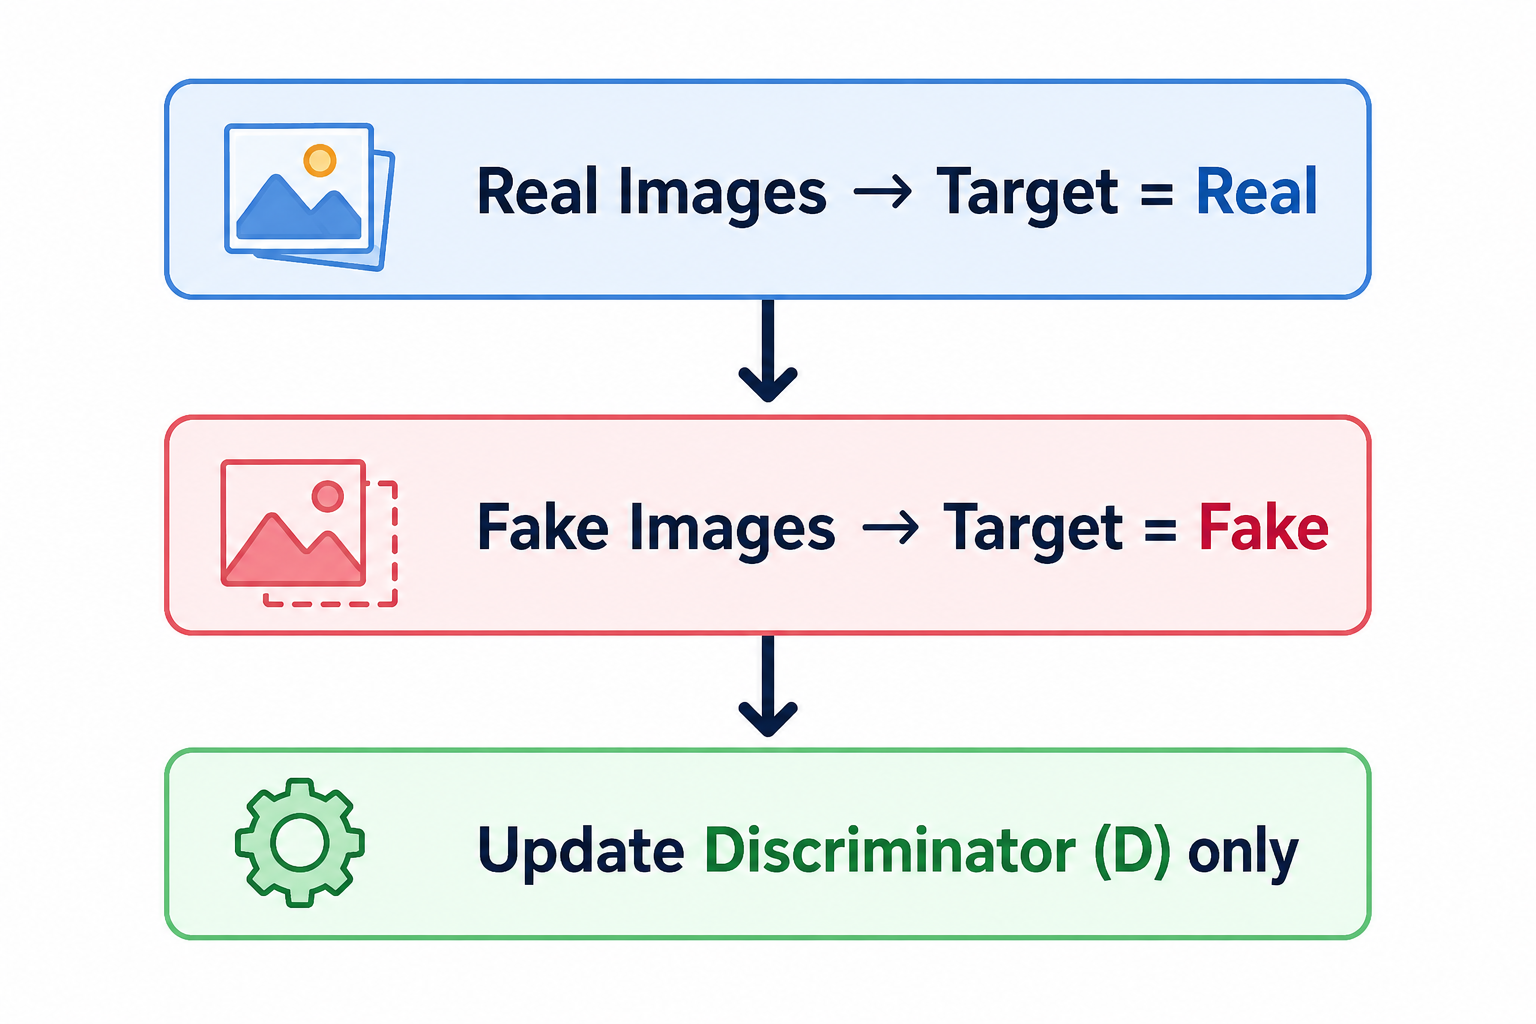
\includegraphics[width=0.85\textwidth]{figures/9-55 figure.png}

\end{figure} 
\clearpage
\subsubsection*{Training the Generator}
\begin{figure}[H]
\centering
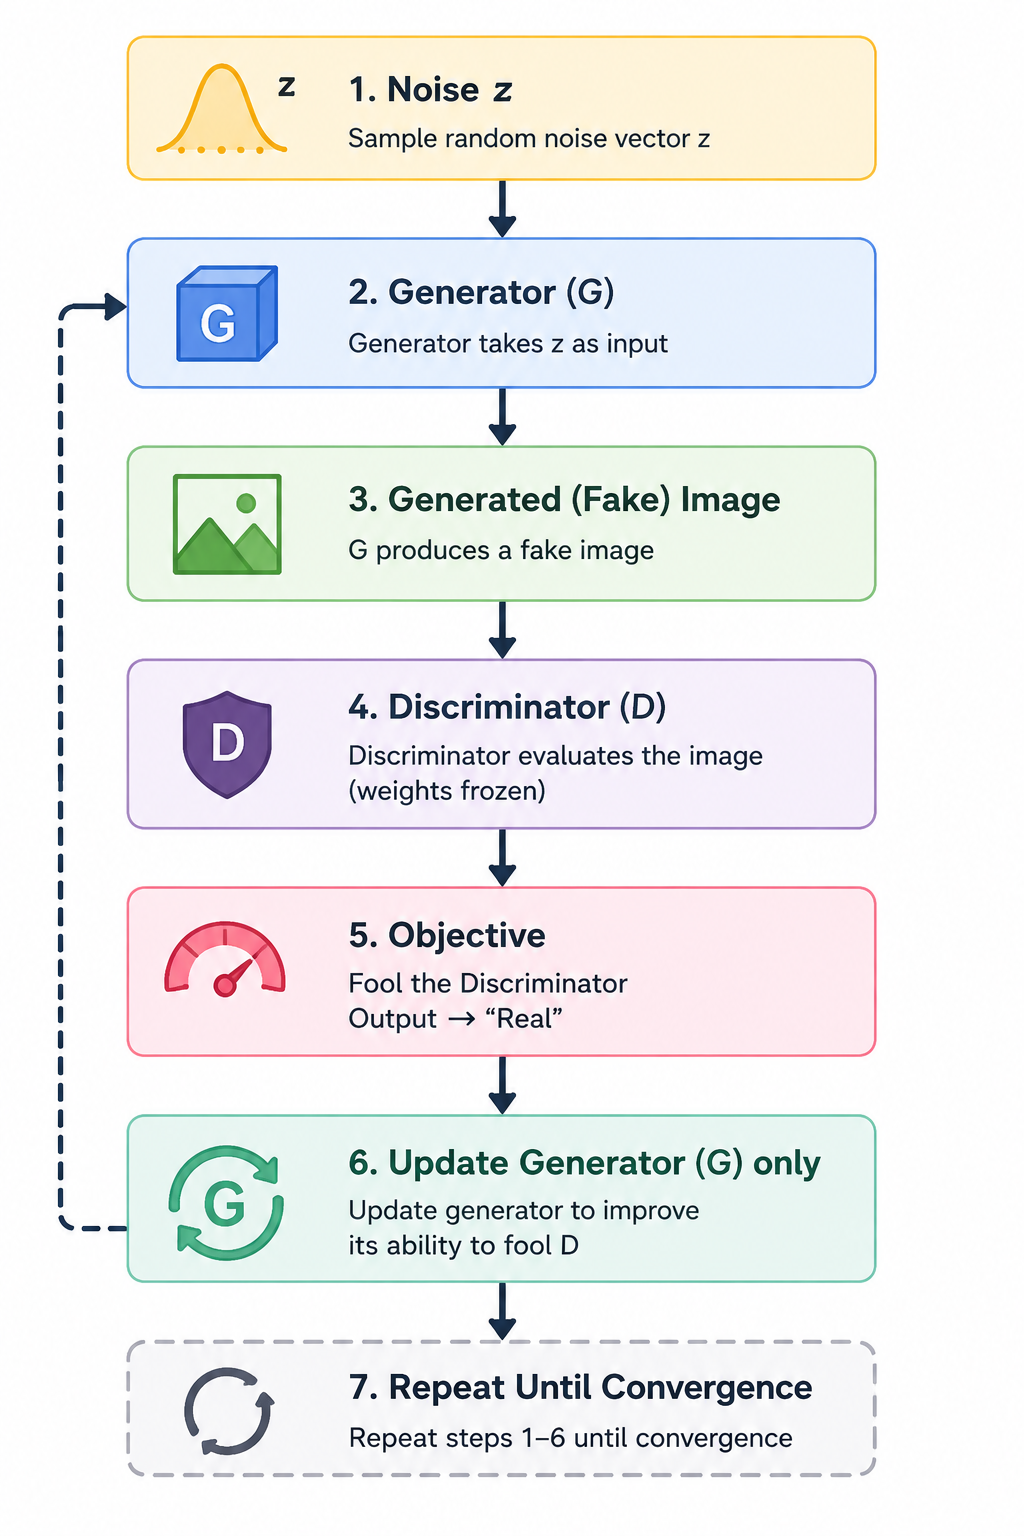
\includegraphics[width=0.85\textwidth]{figures/9-56 figure.png}
\end{figure}

The Generator is Powerful because is never told:
``The left eye should be two pixels higher''
or ``The hair color is wrong''

It receives only one signal: ``This image look fake''
From this simple feedback, it Gradually learns:
\begin{itemize}
    \item facial Structure
    \item lighting
    \item textures
    \item shadows
    \item Object shapes
    \item fine details
\end{itemize}

This is why GANs were able to Produce much sharper images than VAE.

\subsection*{Minimax Game}

GAN Training is formulated as a minimax Game:
\[
\min_G \max_D V(D, G)
\]

\begin{itemize}
    \item Discriminator ($\max_D$) tries to maximize its ability to distinguish real from fake.
    \item Generator ($\min_G$) tries to minimize The Discriminator's success by generating more realistic images.
\end{itemize}

Each network improves by Competing against the other, which is why GANs are called adversarial.

\subsection*{Nash Equilibrium}

The Ideal outcome is The Nash Equilibrium, where:
\begin{itemize}
    \item The Generator produces images indistinguishable from real ones.
    \item The Discriminator Cannot do better than random guessing and outputs approximately $0.5$ for both real and fake images.
\end{itemize}

At this point, neither network can improve its performance without the other changing as well.

In Practice, GANs rarely reach this Perfect balance. One network often becomes stronger than The other, leading To training instability. If the Discriminator becomes too accurate too early, The Generator receives very small gradients (the Vanishing Gradient Problem) and Stop improving. These difficulties Motivated The development of improved GAN variants such as DCGAN, WGAN and StyleGAN.

\section{Why GANs Are Hard to Train}

When GANs were introduced in 2014, they produced amazing images.
But researchers Quickly discovered something frustrating: Training a GAN is much harder than training a CNN, a transformer, or an Autoencoder.
Sometimes it works beautifully. At other times, with the same architecture and almost the same hyperparameters, training completely fails. Why?
Because two neural networks are learning simultaneously, and each one changes the learning environment of the other, making Optimization unstable.

\subsection*{The Four Main Problems}

\subsubsection*{1) Vanishing gradients}
\begin{itemize}
    \item if The Discriminator becomes too good, it Confidently Classifies fake image as fake
    \item The sigmoid output saturates near $0 \sim 0.001$ (fake) or $1$ (real), producing very Small Gradients
    \item As a Result, The Generator receives almost no useful feedback and Stop Learning
\end{itemize}

\subsubsection*{2) Mode Collapse (The most GAN Problem)}

Suppose Our Dataset contains $\begin{cases} \text{- Cats} \\ \text{- Dogs} \\ \text{- Cars} \\ \text{- Birds} \end{cases}$

The Generator should learn all of Them.
If the generator produces a dog image every time, the discriminator is fooled.
The Generator realizes: why should I Generate any thing else?
It starts producing $\text{dog} \rightarrow \text{dog} \rightarrow \text{dog} \dots \rightarrow \text{dog}$ with tiny variations. The generator has found an easy way to fool the discriminator; this phenomenon is called mode collapse.
\begin{itemize}
    \item Instead of learning the entire data distribution (ex: dogs, cats, cars, Birds), The Generator discovers a few Outputs that Consistently fool the Discriminator.
    \item It repeatedly generates only those samples with small variations, ignoring the rest of The data
\end{itemize}

\subsubsection*{3) Oscillation}

Today: the generator learns how to create good cats \\
$\phantom{today:\ }$ the Discriminator adapts \\
Tomorrow: the generator switches to dogs \\
$\phantom{tomorrow:\ }$ the Discriminator adapts again \\
$\phantom{tomorrow:\ } \quad \Downarrow$ \\
$\phantom{tomorrow:\ } \text{Birds} \rightarrow \text{Cats} \rightarrow \text{Dogs} \dots$

The Generator keeps chasing the Discriminator:
\begin{itemize}
    \item The Generator and Discriminator Continually adapt to each other
    \item The Generator may learn to Generate one type of image, The Discriminator adapts, then The Generator Switches to another type
    \item This cycle repeats without reaching a Stable Solution
\end{itemize}

\subsubsection*{4) Imbalanced Learning}
\begin{itemize}
    \item If the Discriminator learns much faster than the Generator, the Generator receives almost no useful Gradients.
    \item If The Generator becomes too Strong, The Discriminator can no longer learn effectively.
    \item Successful GAN training requires both networks to improve at approximately the Same rate.
\end{itemize}

The Original GAN demonstrated that adversarial Learning Could generate highly realistic images, But it Training is inherently unstable due to Vanishing gradients, Mode collapse, oscillation, and Imbalanced Learning. Nearly every later GAN architecture was designed to Address These optimization Challenges while Preserving the Core Generator-versus-Discriminator framework.

\section{DCGAN (Deep Convolutional GAN) (2015)}

Before DCGAN, people Knew GANs worked in Theory but training them on real images was difficult and unstable.
In 2015, DCGAN showed that simply changing the architecture Could dramatically improve image Quality and Training stability.

DCGAN was the first GAN Architecture specifically designed for Image Generation. Instead of Using fully Connected layers like the Original GAN, DCGAN uses Convolutional Neural Network (CNNs), making Training more stable and improving image Quality.

The Original GAN used dense layers, which:
\begin{itemize}
    \item Scale poorly to large images
    \item Ignore spatial relationships between neighboring pixels
    \item Produce lower-Quality images and unstable Training
\end{itemize}

DCGAN solved these issues by replacing dense layers with Convolution-based architecture.

\subsection*{I) Generator Architecture}

The Generator starts from a random noise vector $z$ and progressively increases the image resolution using Transposed Convolution (\textbf{ConvTranspose}).

Each transposed convolution upsamples the feature maps, gradually constructing the final image.

\textbf{why Transposed}: Convolution usually reduces spatial dimensions. $64\times64 \rightarrow \text{Conv} \rightarrow 32\times32$.
A transposed Conv does the opposite: It upsamples the feature maps.
example: $4\times4 \rightarrow \text{TransConv} \rightarrow 8\times8 \rightarrow \text{TransConv} \rightarrow 16\times16\dots$

\begin{figure}[H]
\centering
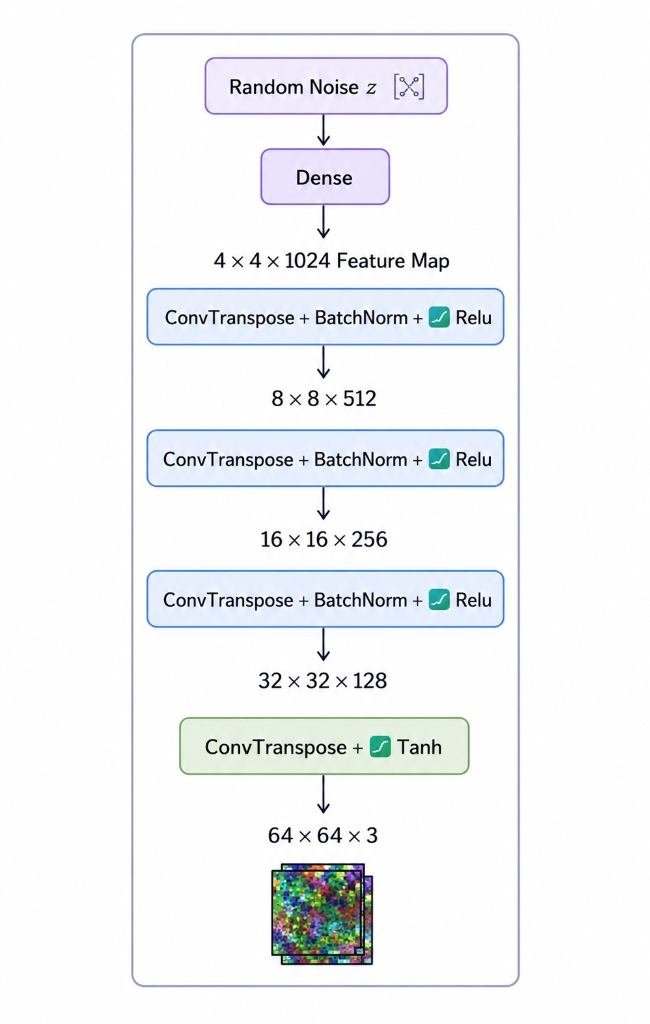
\includegraphics[width=0.88\textwidth]{figures/fig_9_2_dcgan_generator_architecture.jpg}
\end{figure}

\subsection*{II) Discriminator Architecture}

The Discriminator is the mirror of the Generator. It progressively reduces the image size using standard Convolutions, extracts features, and outputs the probability that the image is real.

\begin{figure}[H]
\centering
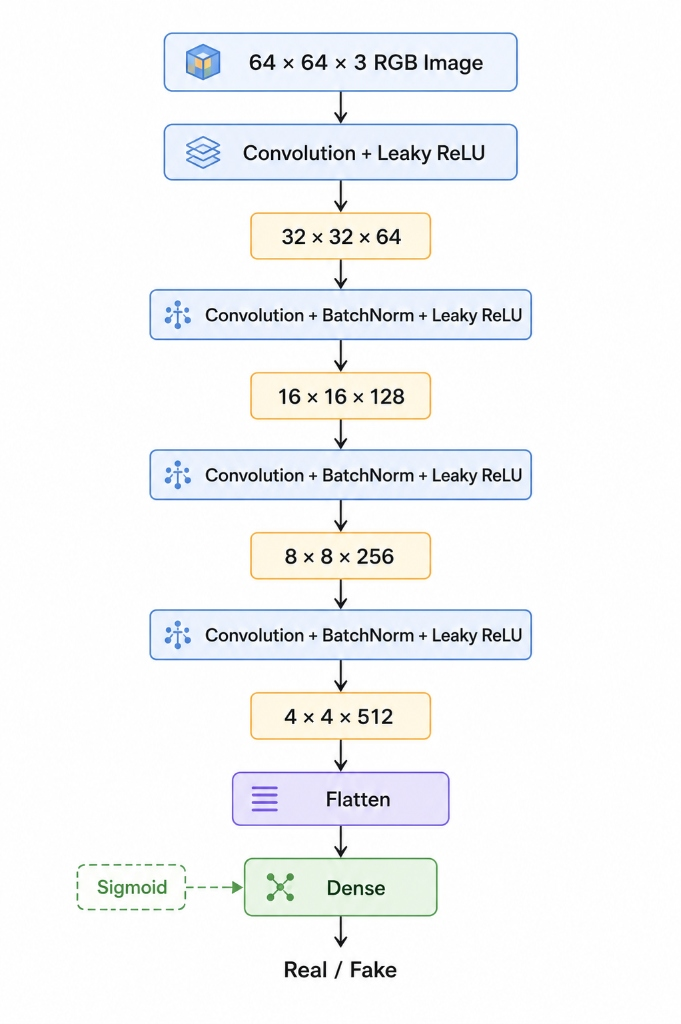
\includegraphics[width=0.88\textwidth]{figures/fig_9_3_dcgan_discriminator_architecture.jpg}
\end{figure}

\subsection*{Overall DCGAN Pipeline}

\begin{figure}[H]
\centering
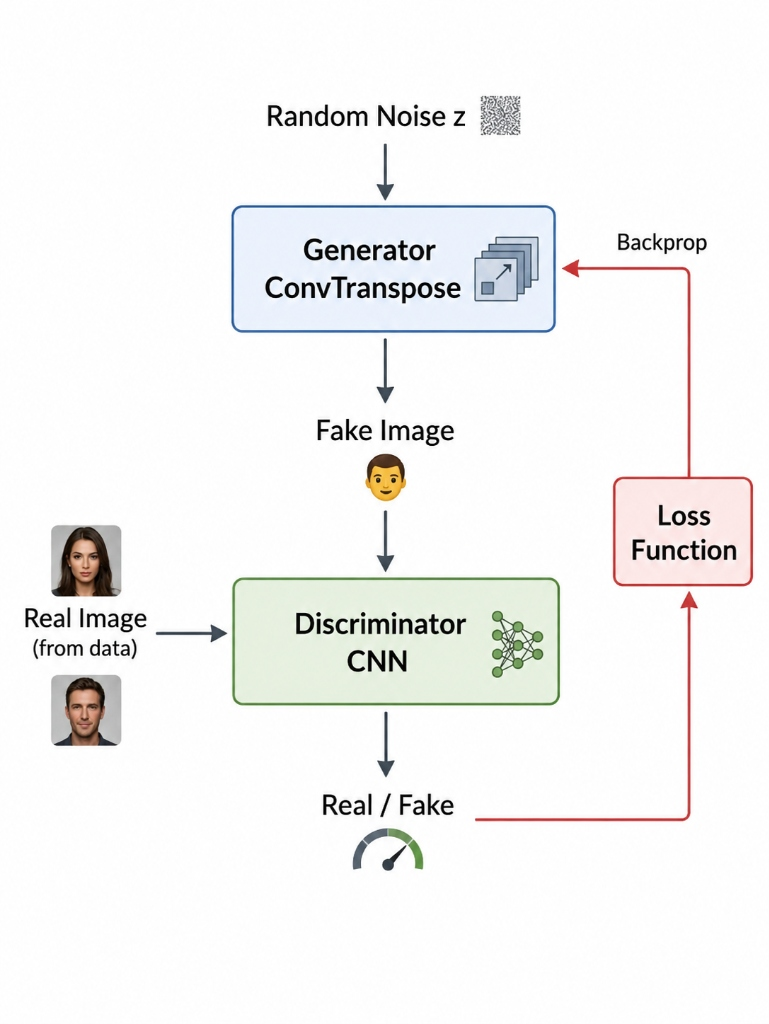
\includegraphics[width=0.88\textwidth]{figures/fig_9_4_overall_dcgan_pipeline.jpg}
\end{figure}

\subsection*{Batch Normalization}

The Original GAN often suffered from unstable Training because activations could change dramatically during optimization, DCGAN introduced Batch Normalization in most layers, BatchNorm helps by:
\begin{itemize}
    \item Stabilizing activations
    \item Speeding up training
    \item making gradient flow more smoothly
\end{itemize}

This does not solve every GAN problem, but it makes optimization much easier.

\subsection*{Leaky ReLU}

The discriminator uses Leaky ReLU instead of ReLU because Leaky ReLU allows a small negative slope. The neuron still receives gradients, which prevents it from stopping learning and improves training stability.

\subsection*{Why Tanh at the Generator Output?}

The generator uses Tanh as its final activation because it outputs pixel values in the range $[-1, 1]$. Therefore, the real training images are also normalized to $[-1, 1]$ so that both real and generated images have the same value range. Matching these ranges helps stabilize training and improves convergence.

\subsection*{DCGAN Design Rules}

\begin{itemize}
    \item Replace pooling layers with strided convolutions (discriminator) and transposed convolutions (generator)
    \item Use Batch Normalization in most layers
    \item Use ReLU in the generator (except the output layer)
    \item Use Leaky ReLU in the discriminator
    \item Use Tanh at the generator output
    \item Remove unnecessary fully connected hidden layers.
\end{itemize}

These simple rules dramatically improved training compared with the original GAN.

DCGAN did not change the adversarial loss. The generator and discriminator still play the same minimax game. The main improvement is the architecture, not the objective.

\section{cGAN Conditional GANs (2016)}

A vanilla GAN generates images randomly.
\[
\text{Noise } (z) \longrightarrow \text{Generator} \longrightarrow \text{Random Image}
\]

We cannot control whether the output is a dog, cat, car, or house. Imagine asking a GAN, ``Generate a cat.'' It cannot; it only maps noise to images.

A conditional GAN (cGAN) adds extra information (a condition) to both the generator and the discriminator. Usually, the condition is a class label.

Researchers asked: what if we also give the Generator the class label?
Instead of Noise $\rightarrow$ Generator $\rightarrow$ Image, we use:
\[
\text{Noise} + \text{Label} \longrightarrow \text{Generator} \longrightarrow \text{Image}
\]

Now the generator knows:
\begin{itemize}
    \item The random appearance ($z$)
    \item The desired category (label)
\end{itemize}

\subsection*{Generator}

Instead of receiving only $z$, the generator receives $(z, y)$, where $z = \text{random noise}$ and $y = \text{label}$.

\[
z + \text{Label} = \text{dog} \longrightarrow \text{Generator} \longrightarrow \text{Random dog}
\]

\begin{itemize}
    \item The label controls what is generated.
    \item The noise controls how it looks.
\end{itemize}

Why keep the noise? Suppose the generator receives only ``dog.'' Then every output would become dog A, dog A, dog A: always the same dog.
The noise introduces diversity:
\[
\left.
\begin{array}{l}
z_1 + \text{Dog} \longrightarrow \text{Dog a} \\
z_2 + \text{Dog} \longrightarrow \text{Dog b} \\
z_3 + \text{Dog} \longrightarrow \text{Dog c}
\end{array}
\right\} \quad \text{Same class, different appearance}
\]

\subsection*{Discriminator}

The discriminator now receives an image plus a label. Instead of asking ``real or fake?'', it asks, ``Is this image real for this label?''
Even if the image is real, the discriminator rejects it when it does not match the condition.

\begin{figure}[H]
\centering
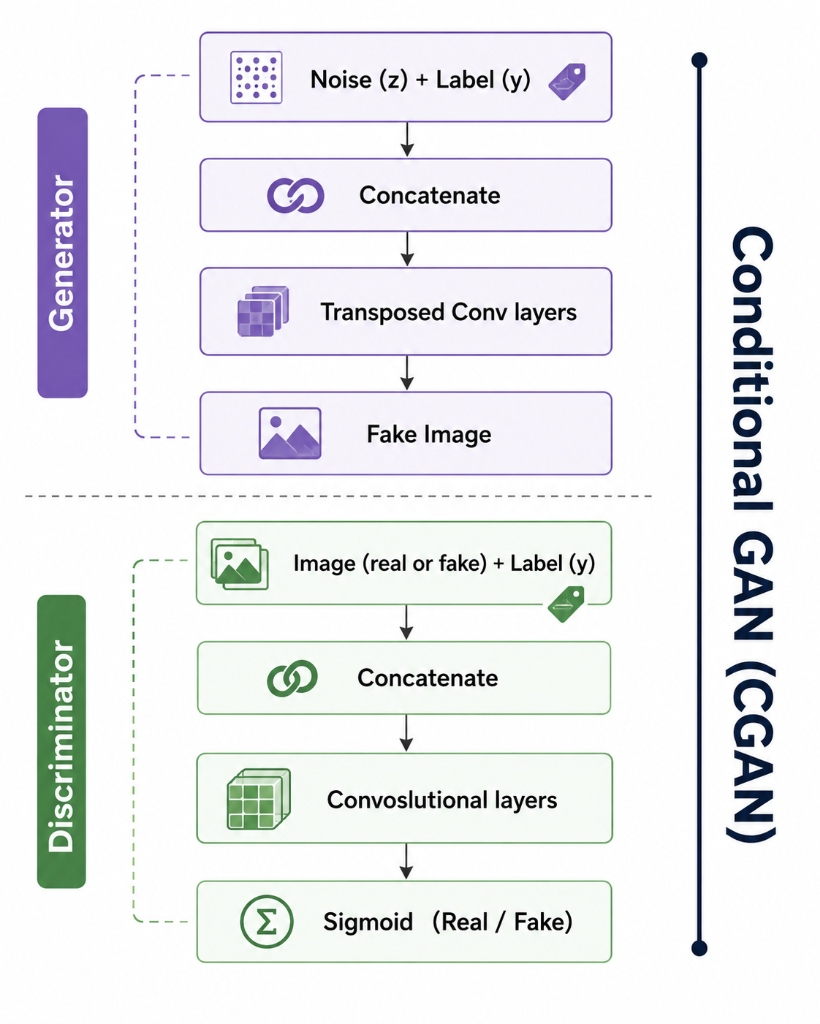
\includegraphics[width=0.88\textwidth]{figures/fig_9_5_cgan_architecture.jpg}
\end{figure}

\subsection*{Training Flow}

\begin{enumerate}
    \item Choose a label $y$ (ex: dog)
    \item Sample random noise $z$.
    \item Generator: $(z, y) \rightarrow \text{fake dog}$.
    \item Discriminator: $(\text{real dog}, y) \rightarrow \text{real}$.
    \item Discriminator: $(\text{fake dog}, y) \rightarrow \text{fake}$.
    \item Update the discriminator.
    \item Freeze the discriminator.
    \item Generate another fake dog using $(z, y)$.
    \item Update the generator so the discriminator predicts ``real.''
    \item Repeat
\end{enumerate}

\subsection*{Applications}

\begin{itemize}
    \item Image Generation
    \item Image Colorization
    \item Super Resolution
    \item Semantic Image Generation
\end{itemize}

\section{Pix2Pix}

Pix2Pix is one of the most influential Conditional Generative Adversarial Networks (cGANs). Instead of conditioning the generator on a class label, Pix2Pix conditions both the generator and discriminator on an input image. The model learns a mapping from the input image to a corresponding output image, enabling \textbf{image-to-image translation} tasks such as image colorization, semantic segmentation, edge-to-photo synthesis, and style transformation.

\subsection*{Limitation of Pix2Pix}


\section{CycleGAN: Unpaired Image-to-Image Translation (2017)}

Unlike models that require fully paired and matched data (such as Pix2Pix), CycleGAN enables us to learn from completely independent datasets. In many real-world applications, collecting such paired data is nearly impossible, which is why CycleGAN comes as an alternative solution.

Instead of relying on precise matching between images, CycleGAN learns from two independent and distinct sets of images:
\begin{itemize}
    \item \textbf{Domain A (Dataset 1)}: e.g., Horse Domain
    \item \textbf{Domain B (Dataset 2)}: e.g., Zebra Domain
\end{itemize}

\begin{figure}[H]
\centering
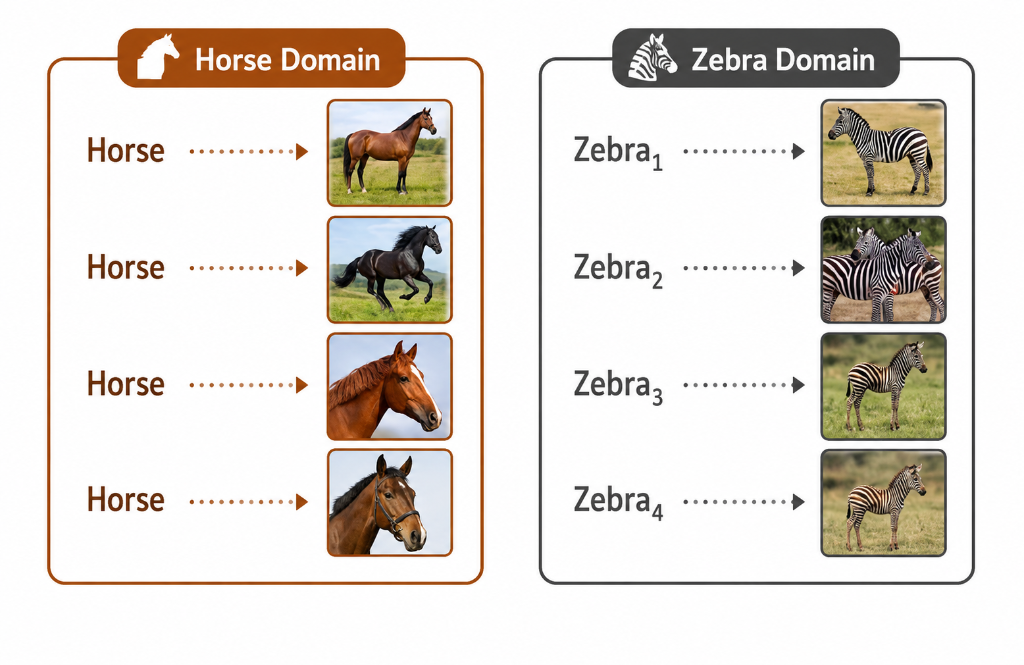
\includegraphics[width=0.85\textwidth]{figures/fig_9_12_cyclegan_domains.png}
\caption{Unpaired Domain Mapping: Horse Domain ($X$) vs. Zebra Domain ($Y$).}
\label{fig:cyclegan_domains}
\end{figure}

Thus, the model only knows that these images belong to the Horse Domain and those images are associated with the Zebra Domain.

\subsection*{Dual Generator and Discriminator Architecture}

Suppose we have a Horse image and Generator $G$ turns it into a Zebra. But how do we know if it looks like a Zebra while preserving the pose, background, and shape of the original horse? It could generate any random Zebra!

Solution: CycleGAN introduces two Generators instead of one:
\begin{itemize}
    \item \textbf{Generator $G$}: Learns the mapping from Domain A to Domain B ($A \rightarrow B$, e.g., Horse $\rightarrow$ Zebra).
    \item \textbf{Generator $F$}: Learns the mapping from Domain B to Domain A ($B \rightarrow A$, e.g., Zebra $\rightarrow$ Horse).
    \item \textbf{Discriminator $D_B$}: Evaluates whether an image in Domain B is real or generated by $G$.
    \item \textbf{Discriminator $D_A$}: Evaluates whether an image in Domain A is real or generated by $F$.
\end{itemize}

\begin{figure}[H]
\centering
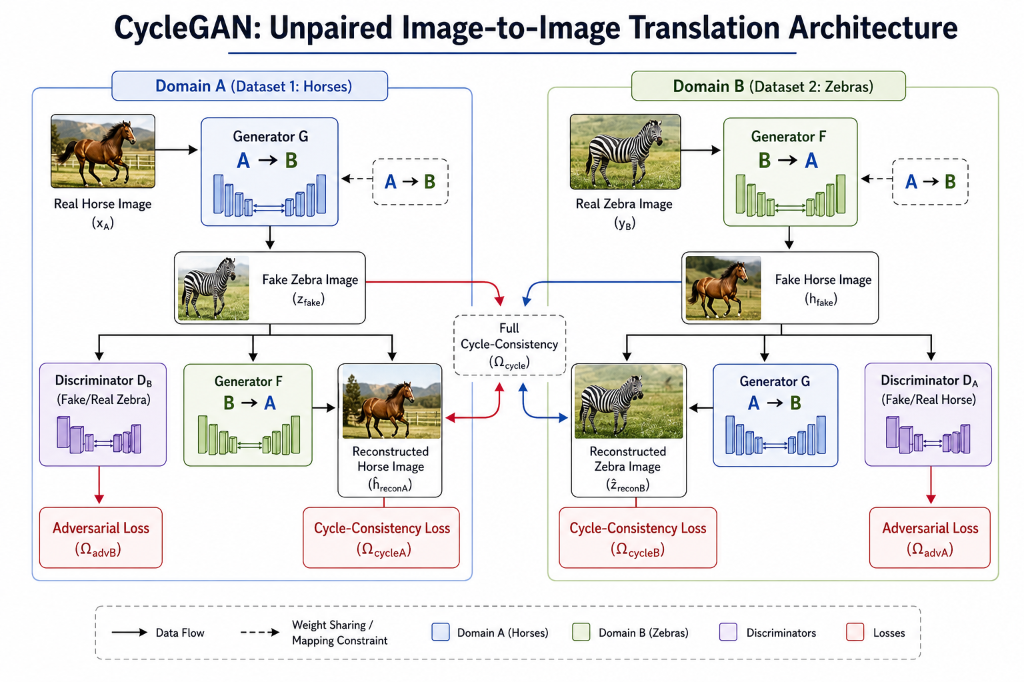
\includegraphics[width=0.92\textwidth]{figures/fig_9_13_cyclegan_architecture.png}
\caption{CycleGAN Complete Dual-Generator Architecture and Loss Interactions.}
\label{fig:cyclegan_arch}
\end{figure}

\subsection*{Cycle Consistency}

First, an image from Domain A is translated by Generator $G$ into a fake image in Domain B. Instead of stopping there, this generated image is passed through Generator $F$ to translate it back into Domain A. If the translation is meaningful, the reconstructed image should closely resemble the original input.

In other words, translating an image from one domain to another and then back again should recover the original image. The same process is performed in the opposite direction (Domain B $\rightarrow$ Domain A $\rightarrow$ Domain B).

By minimizing the difference between the original and reconstructed images, CycleGAN encourages the generators to preserve the content, structure, and identity of the image while changing only the domain-specific characteristics, allowing image-to-image translation without requiring paired training examples.

\subsection*{Why Does Cycle Consistency Work?}

Imagine we hire a translator: $\text{English} \longrightarrow \text{French} \longrightarrow \text{English}$. If the final English sentence is very different, the translation was poor. But if we recover almost the same sentence, the translation preserved the meaning. CycleGAN applies exactly the same principle to images.

Before CycleGAN, image-to-image translation required expensive paired datasets. CycleGAN showed that consistency is enough. Instead of saying ``this horse corresponds to this zebra'', it says ``if I translate there and back, I should recover the original.''

That simple idea removed the need for paired training examples.

\subsection*{CycleGAN Training Pipeline}

\begin{figure}[H]
\centering
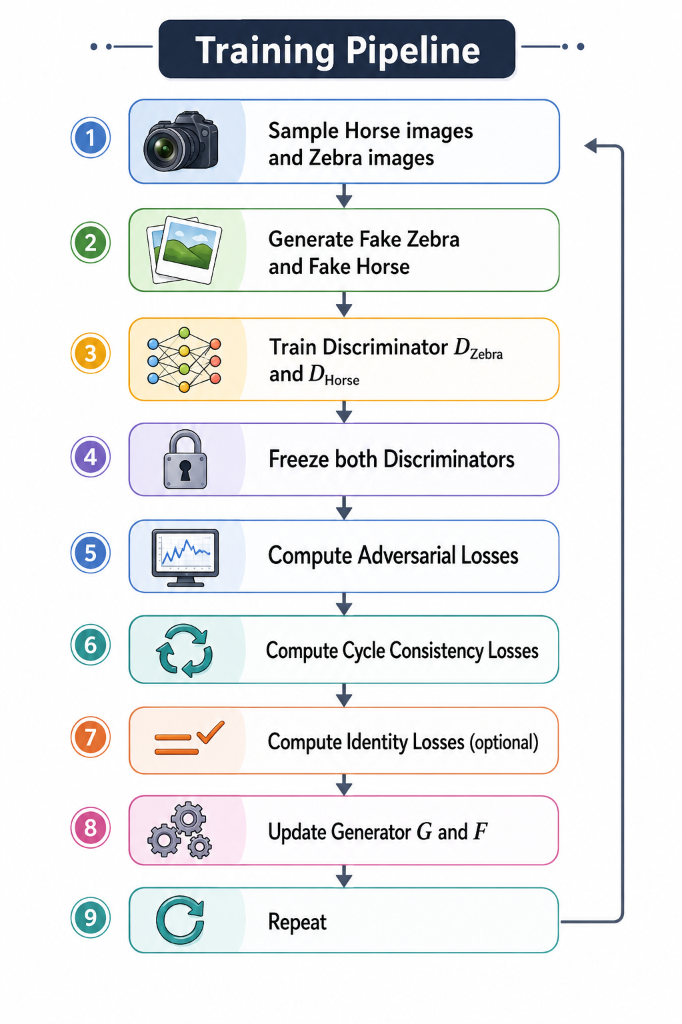
\includegraphics[width=0.78\textwidth]{figures/fig_9_14_cyclegan_pipeline.png}
\caption{CycleGAN Step-by-Step Training Pipeline.}
\label{fig:cyclegan_pipeline}
\end{figure}

This alternating process enables CycleGAN to learn realistic unpaired image-to-image translations while preserving original image content through Cycle Consistency.

\subsection*{The Three Losses in CycleGAN}

Unlike a vanilla GAN, CycleGAN does not rely on a single loss function; it combines three objectives:

\subsubsection*{1) Adversarial Loss}

Exactly like a normal GAN, Generator $G$ tries to fool the Zebra Discriminator ($D_B$), and Generator $F$ tries to fool the Horse Discriminator ($D_A$).

\subsubsection*{2) Cycle Consistency Loss}

This is the core loss:
\[
\text{Horse} \longrightarrow \text{Zebra} \longrightarrow \text{Horse} \approx \text{Original Horse}
\]
The reconstructed horse should remain close to the input image $x$:
\[
F(G(x)) \approx x \quad \text{and} \quad G(F(y)) \approx y
\]
\[
\mathcal{L}_{\text{cyc}}(G, F) = \mathbb{E}_{x \sim P_{\text{data}}(x)}[\|F(G(x)) - x\|_1] + \mathbb{E}_{y \sim P_{\text{data}}(y)}[\|G(F(y)) - y\|_1]
\]

\subsubsection*{3) Identity Loss (Optional but Very Useful)}

Identity loss teaches the generator not to change an image that is already in the target domain.

Generator $G$ is trained to convert Horse $\rightarrow$ Zebra. Now imagine that during training, we purposely give Generator $G$ a Zebra instead of a Horse. What should the output be?
\[
\text{Zebra} \longrightarrow \text{Generator } G \longrightarrow \text{Zebra}
\]
By passing a Zebra into Generator $G$, we are basically telling the Generator: ``This image is already in your target domain. Don't touch it.''

Identity loss helps preserve color composition and visual tone across domain translations.

\subsection*{Limitations of CycleGAN}
\begin{enumerate}
    \item \textbf{Cannot change geometry well}: It works best when the two domains have similar shapes (e.g., Horse $\rightarrow$ Zebra $\checkmark$, but Cat $\rightarrow$ Airplane $\times$).
    \item \textbf{May change important details}: It can unintentionally modify background colors or object identity.
    \item \textbf{Cycle consistency is not a guarantee}: An image can satisfy the cycle loss while still producing an unrealistic translation.
    \item \textbf{Training is slow and unstable}: It trains two generators and two discriminators simultaneously, making optimization difficult.
    \item \textbf{Requires enough data from both domains}: Although paired images are unnecessary, we still need a large collection of images from each domain.
\end{enumerate}

\begin{itemize}
    \item \textbf{Strength}: No paired dataset is required.
    \item \textbf{Weakness}: It struggles with large structural changes and still inherits the training instability common to GANs.
\end{itemize}

\section{StyleGAN (2019)}

In a normal GAN, the random latent vector $z$ is fed directly into the Generator to produce an image. Ideally, changing one part of $z$ should modify only one visual attribute, such as hair color or age. However, this is not what happens in practice. The latent space is \textbf{entangled}, meaning that information for different attributes is mixed together.

As a result, a small change in $z$ can simultaneously affect several characteristics of the generated image, such as age, hairstyle, lighting, face, or even background.

\begin{figure}[H]
\centering
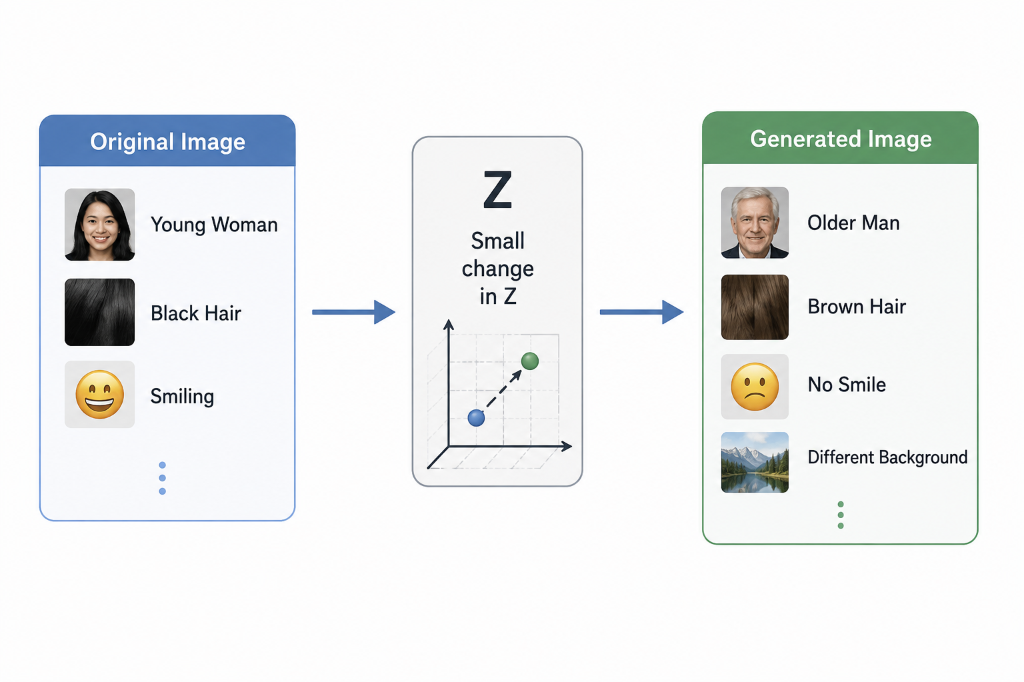
\includegraphics[width=0.85\textwidth]{figures/fig_9_11_latent_space_z.png}
\caption{Entangled Latent Space $Z$: Small changes in $Z$ affect multiple unrelated visual attributes.}
\label{fig:latent_z}
\end{figure}

Instead of changing only one attribute, many unrelated attributes change together. This lack of independent control makes it difficult to edit generated images in a meaningful and predictable way. StyleGAN was designed to solve this problem by learning a more \textbf{disentangled latent space}, where different directions correspond to different visual attributes.

\subsection*{StyleGAN: Key Innovations (2019)}

\textbf{The Main Idea}: Instead of sending $z$ directly into the Generator, StyleGAN first transforms it.

\begin{figure}[H]
\centering
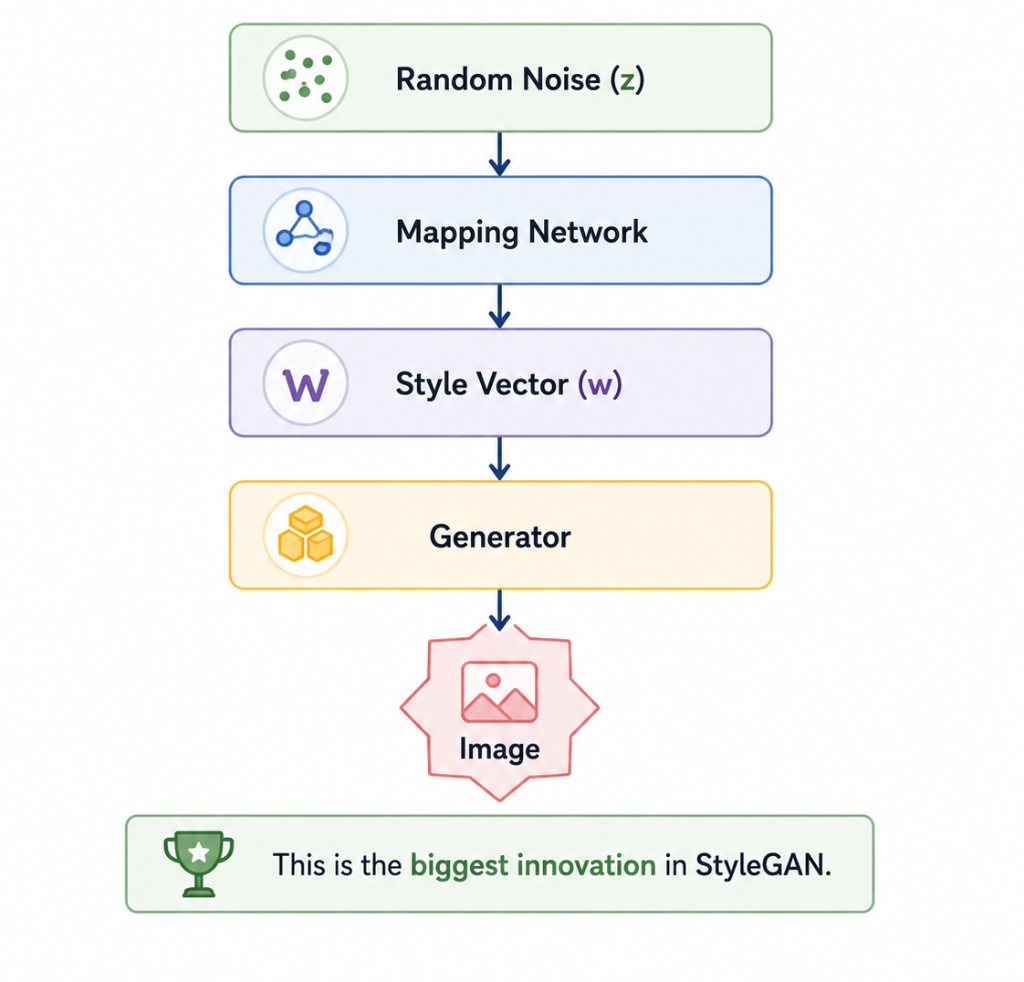
\includegraphics[width=0.82\textwidth]{figures/fig_9_7_stylegan_mapping_network.png}
\caption{StyleGAN Mapping Network ($z \rightarrow w$) Innovation.}
\label{fig:stylegan_mapping}
\end{figure}

This is the biggest innovation in StyleGAN.

\subsection*{I) Mapping Network}

The Mapping Network is a small MLP (typically 8 fully connected layers). Its job is:
\[
z \longrightarrow \text{Mapping Network} \longrightarrow w
\]
Where $z$ is the original random latent vector, and $w$ is the new latent representation.

$z$ comes from a simple Gaussian distribution $z \sim \mathcal{N}(0, I)$. Nothing in this distribution specifies separate dimensions (e.g., dimension 5 for hair color, dimension 12 for smile). The Generator must learn everything at once. The Mapping Network reorganizes this space into one that is easier for the Generator to use.

The goal is to make $w$ much more disentangled: instead of mixing all attributes together, different directions in $w$ tend to correspond to meaningful visual properties like age, hairstyle, pose, or facial expression.

\subsection*{II) Adaptive Instance Normalization (AdaIN)}

This is the second major innovation. Instead of using the same feature statistics for every generated image, \textbf{AdaIN} modifies the feature maps according to the style vector $w$. This allows each layer of the Generator to control different visual attributes (pose, hairstyle, colors...):

\[
\text{AdaIN}(x, w) = \gamma(w) \left( \frac{x - \mu(x)}{\sigma(x)} \right) + \beta(w)
\]

Where $x$ is the feature map, $\gamma(w)$ is the learned scale from the style vector, and $\beta(w)$ is the learned shift from the style vector.

\begin{figure}[H]
\centering
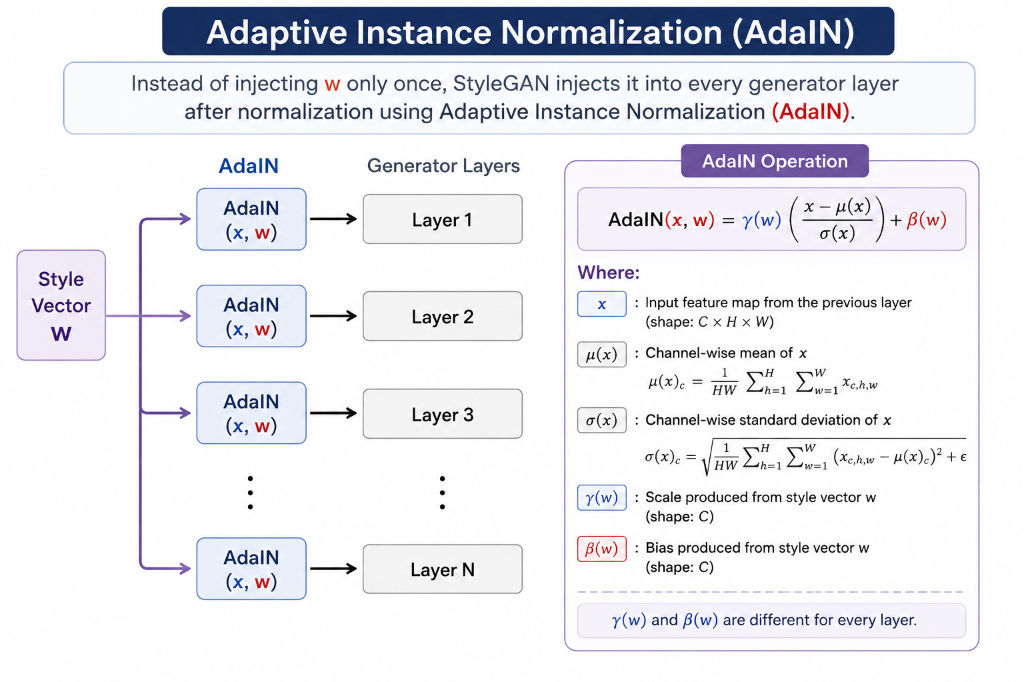
\includegraphics[width=0.88\textwidth]{figures/fig_9_8_adain_operation.png}
\caption{Adaptive Instance Normalization (AdaIN) Operation and Mathematical Formulation.}
\label{fig:adain_op}
\end{figure}

Different layers control different image properties:
\begin{itemize}
    \item \textbf{Early layers ($4\times4 - 8\times8$)}: Pose, face shape, coarse structure.
    \item \textbf{Middle layers ($16\times16 - 64\times64$)}: Eyes, nose, mouth, hairstyle.
    \item \textbf{Late layers ($128\times128 - 1024\times1024$)}: Skin texture, wrinkles, pores, fine details.
\end{itemize}

Instead of one global latent vector controlling everything, StyleGAN allows each layer to receive style independently.

\subsection*{Progressive Image Formation}

The image is generated from coarse to fine (e.g., the head first, then eyes/nose, and finally hair, skin texture, and tiny details):
\[
\text{Low Resolution} \longrightarrow \text{Overall Structure} \longrightarrow \text{Medium Resolution} \longrightarrow \text{Facial Features} \longrightarrow \text{High Resolution} \longrightarrow \text{Fine Details}
\]

\subsection*{III) Style Mixing \& Noise Injection}

\subsubsection*{Style Mixing}

Suppose we have two latent vectors:
\begin{itemize}
    \item $w_1 \rightarrow$ young woman
    \item $w_2 \rightarrow$ old man
\end{itemize}
Instead of using one style vector for every layer, we can combine them:
\begin{itemize}
    \item \textbf{Early layers}: $w_1$
    \item \textbf{Late layers}: $w_2$
\end{itemize}
$\Rightarrow \textbf{Result}$: Young face $+$ Old skin texture. Different parts of the Generator can receive different styles. This was impossible in earlier GANs.

\subsubsection*{Noise Injection}

Another innovation is per-layer random noise. StyleGAN adds small random noise inside each layer:
\[
\text{Feature Map} + \text{Noise} \longrightarrow \text{Next Layer}
\]
\begin{itemize}
    \item \textbf{Effect}: Very small stochastic details (freckles, skin pores, tiny hair strands, wrinkles).
    \item \textbf{$w$}: Controls the overall style.
    \item \textbf{Noise}: Controls tiny random variations.
\end{itemize}

\subsection*{IV) Learned Constant Tensor \& Generator Blocks}

Unlike previous GANs, the Generator does not start from $z$. Instead, it starts from a \textbf{Learned Constant Tensor} ($4\times4\times512$) that is learned during training and serves as the initial feature map.

\begin{figure}[H]
\centering
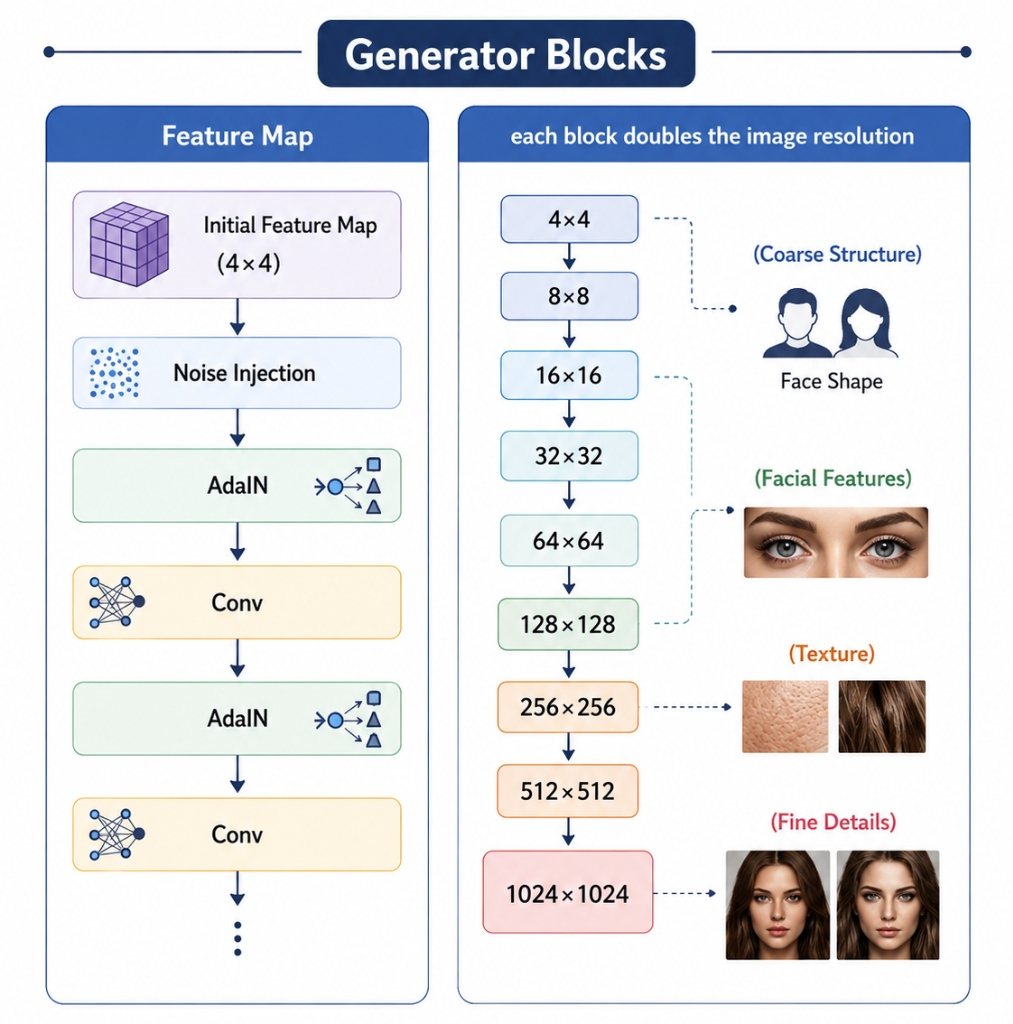
\includegraphics[width=0.88\textwidth]{figures/fig_9_9_stylegan_generator_blocks.png}
\caption{StyleGAN Generator Blocks and Multi-Scale Feature Resolution Control.}
\label{fig:stylegan_blocks}
\end{figure}

\begin{figure}[H]
\centering
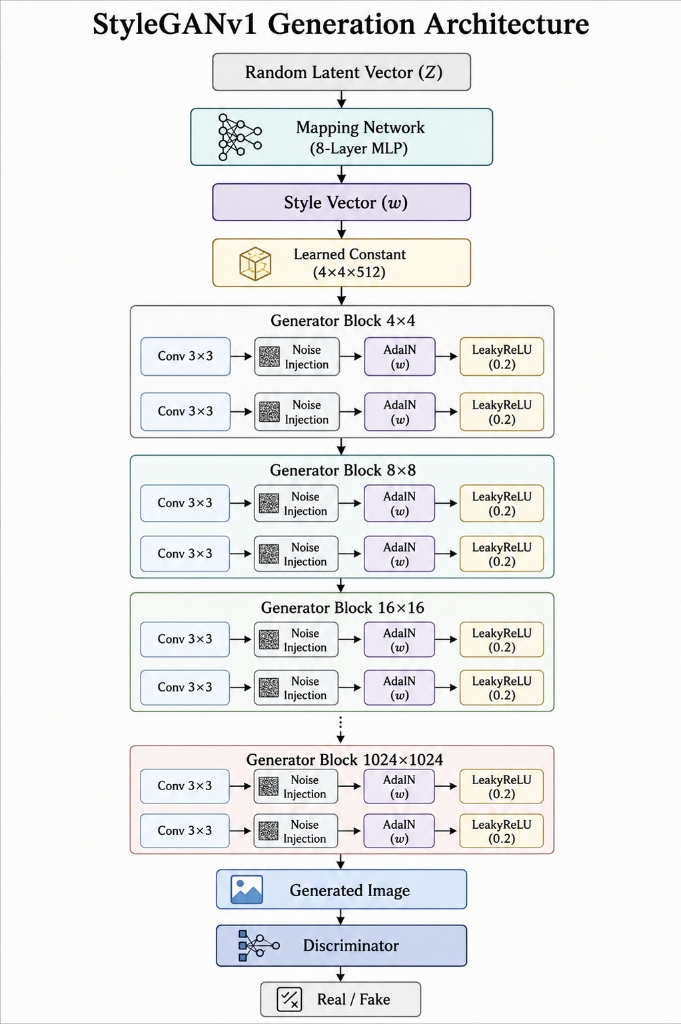
\includegraphics[width=0.88\textwidth]{figures/fig_9_10_stylegan_architecture.png}
\caption{Full StyleGANv1 Generation Pipeline and Discriminator Topology.}
\label{fig:stylegan_full}
\end{figure}

\subsection*{StyleGAN Advantages}

StyleGAN was revolutionary because for the first time, researchers could modify a generated face in a meaningful way (e.g., smile $\rightarrow$ increase, age $\rightarrow$ older, hair $\rightarrow$ longer, pose $\rightarrow$ rotate head) without changing everything else.

\begin{itemize}
    \item Disentangled latent space.
    \item Easy attribute manipulation.
    \item Different layers control different visual features.
    \item Highly realistic textures.
    \item Fine-grained control over generated images.
\end{itemize}

\section{WGAN (Wasserstein GAN) (2017)}

\begin{itemize}
    \item Original GAN suffers from vanishing gradients when the Discriminator becomes too strong.
    \item WGAN replaces the original loss function with the \textbf{Wasserstein (Earth Mover's) Distance}, providing a more useful learning signal.
\end{itemize}

\textbf{Main Idea}: Instead of classifying images as real or fake, WGAN measures how far the generated data distribution is from the real data distribution.
\begin{itemize}
    \item \textbf{Original GAN}: Discriminator $\rightarrow$ Probability ($0$ to $1$).
    \item \textbf{WGAN}: Critic $\rightarrow$ Real-valued score ($-\infty$ to $+\infty$).
\end{itemize}

The goal is to minimize the Wasserstein distance between the real and generated distributions:

\[
\begin{array}{ccc}
\textbf{Original GAN} & & \textbf{WGAN} \\
\text{Image} & & \text{Image} \\
\downarrow & & \downarrow \\
\text{Discriminator} & & \text{Critic} \\
\downarrow & & \downarrow \\
\text{Probability (Real/Fake)} & & \text{Real-valued Score}
\end{array}
\]

The architecture is almost the same as a GAN; the main differences are the loss function and replacing the Discriminator with a Critic.

WGAN improves GAN training by replacing the Discriminator with a Critic that outputs a real-valued score instead of a probability. It optimizes the Wasserstein (Earth Mover's) distance:
\[
W(P_r, P_g) = \inf_{\gamma \in \Pi(P_r, P_g)} \mathbb{E}_{(x,y) \sim \gamma}[\|x - y\|]
\]
Where $P_r$ is the real data distribution, $P_g$ is the generated data distribution, $\|x - y\|$ is the distance (cost) of moving one unit of mass from $x$ to $y$, and $\inf$ is the minimum over all possible transport plans.

This measures how far the generated data distribution is from the real data distribution, providing meaningful gradients throughout training even when generated images are initially poor. It results in more stable and reliable training with a much lower risk of vanishing gradients.

WGAN does not classify images (no Sigmoid $[0,1]$). Instead, the Critic assigns any real-valued score.

\begin{figure}[H]
\centering
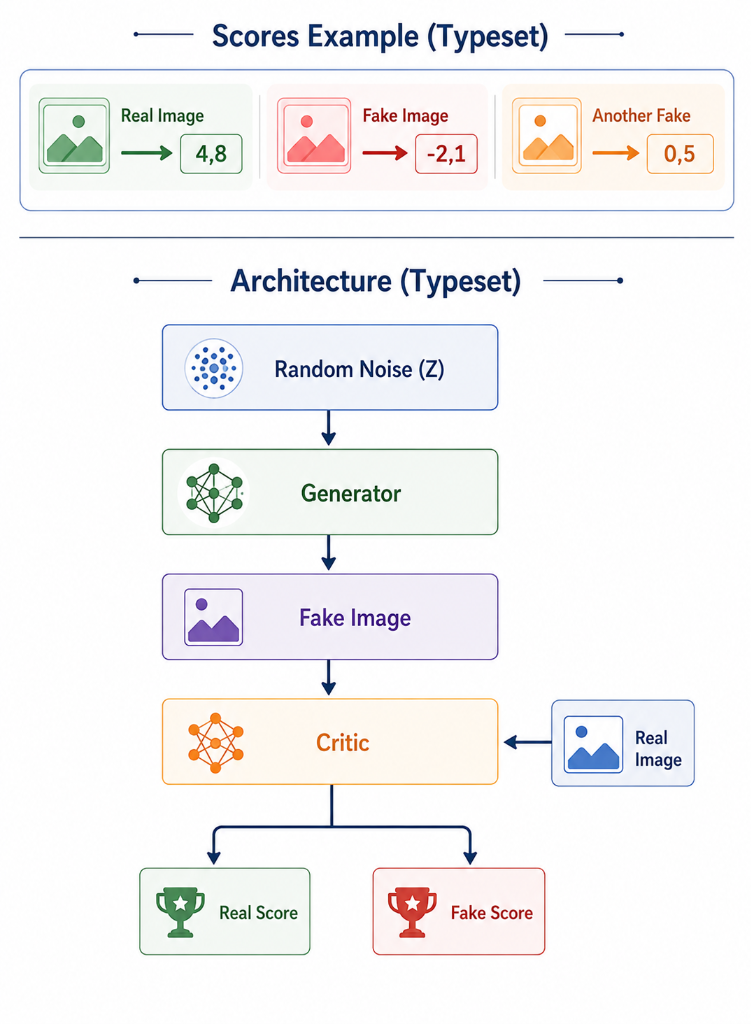
\includegraphics[width=0.88\textwidth]{figures/fig_9_6_wgan_architecture.png}
\caption{WGAN Critic Architecture and Scoring Mechanism.}
\label{fig:wgan_architecture}
\end{figure}

\subsection*{Weight Clipping}

After every update, the Critic's weights are forced into a small range e.g. $[-0.01, 0.01]$. This satisfies the requirement for the Wasserstein distance. However, clipping has drawbacks:
\begin{itemize}
    \item Reduces model capacity.
    \item Makes optimization harder.
    \item Can lead to poor performance.
\end{itemize}

\subsection*{WGAN-GP (Gradient Penalty)}

Researchers quickly improved WGAN by replacing weight clipping with a \textbf{Gradient Penalty (GP)}. Instead of forcing the weights to stay small, they directly penalize the gradients when they become too large.

\subsubsection*{Benefits}
\begin{itemize}
    \item More stable training.
    \item Better image quality.
    \item Easier optimization.
\end{itemize}

\subsubsection*{Limitations}
\begin{itemize}
    \item WGAN-GP is computationally more expensive because of the gradient penalty.
    \item It does not solve problems like controllability or image editing.
    \item It still inherits the complexity of adversarial training.
\end{itemize}

\section{BigGAN (2018)}

Researchers noticed an interesting trend:
\begin{itemize}
    \item As CNNs became larger $\longrightarrow$ performance improved.
    \item As Transformers became larger $\longrightarrow$ performance improved.
\end{itemize}
So they asked: what happens if we simply build a much bigger GAN? That idea led to BigGAN (2018).

Previous GANs were usually trained on CelebA, LSUN, or CIFAR-10. These datasets are relatively small. BigGAN was designed for ImageNet, which contains over 1 million images across 1000 object classes. Training a GAN on ImageNet was considered extremely difficult because the dataset is much larger, there are many object categories, and images are far more diverse.

\subsection*{Key Architectural \& Training Innovations in BigGAN}

\textbf{Main Idea}: BigGAN did not invent a completely new architecture; instead, it combined several good ideas:
\begin{itemize}
    \item Conditional GAN (control the class).
    \item Deeper and wider networks.
    \item Residual Blocks (ResNet).
    \item Large batch sizes.
    \item Spectral Normalization for stable training.
\end{itemize}
The philosophy was to scale everything up.

BigGAN demonstrated that scaling works. Simply making the models larger, training on more data, and using stable training techniques produced a huge leap in image quality. Generated images became sharper, more detailed, more diverse, and closer to real photographs.

\subsection*{Limitations of BigGAN}
\begin{itemize}
    \item Requires massive computational resources (often multiple high-end GPUs or TPUs).
    \item Training is expensive and time-consuming.
    \item Mainly designed for class-conditional image generation.
    \item Less flexible for image editing than StyleGAN.
\end{itemize}

\section{StyleGAN2 (2020) \& StyleGAN3 (2021)}

\subsection*{StyleGAN2 (2020)}

StyleGAN2 improved the original StyleGAN by removing visual artifacts (unwanted patterns or defects) and producing sharper, more realistic images. It redesigned parts of the Generator, leading to better image quality, smoother latent space interpolation, and more stable training. StyleGAN2 became the standard architecture for high-quality face generation.

\subsection*{StyleGAN3 (2021)}

StyleGAN3 focused on eliminating aliasing artifacts, making generated images more geometrically consistent. In StyleGAN2, small changes in the latent vector could cause textures (like hair or skin) to appear ``stuck'' to the image. StyleGAN3 solved this by making features move naturally with objects, producing more realistic animations and transformations.
